\section{Failure Modes \label{sec:fail}}


\begin{enumerate}
    \item \textbf{Misinterpretation of depth} - One of the most common failure cases of the encoder perception pipeline is the misinterpretation of the depth. As shown in the figures at 
    \ref{fig:scenes}, the gripper orients itself correctly and position just a bit higher than the targeted object. After positioning, it attempts to grasp the object but fails because of the height difference between the object and gripper. This scenario occurs more frequently in the test dataset than the training set. The agent can overcome this failure case by understanding that the encoder is yielding wrong information, and it needs to go further down to grasp the object. However, since it does not know the test objects, it tries the standard grasp policy but fails because of the discrepancy between encoded depth and real depth. That is the reason why the encoder converged to a lower success rate than the depth.
        % \begin{figure}[!htbp]
        %     \begin{subfigure}{0.49\textwidth}
        %         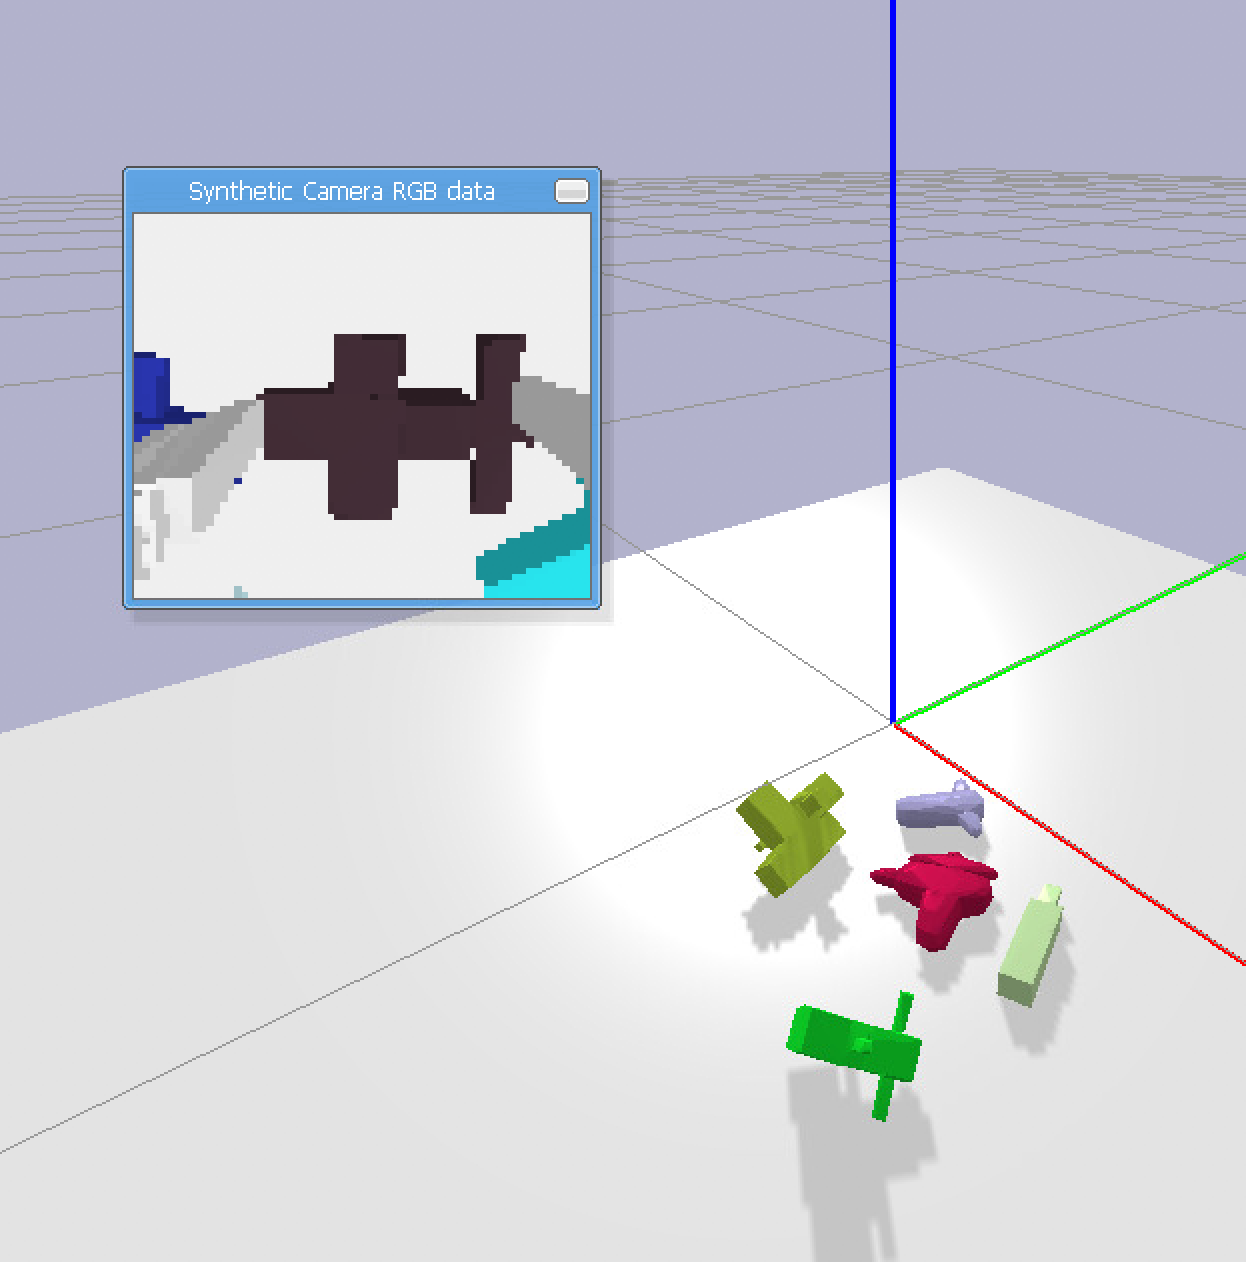
\includegraphics[width=\linewidth]{figures/failure/floorfailure1}
        %         \caption{Table Scene} \label{fig:table}
        %     \end{subfigure}%
        %     \hspace*{\fill}   % maximize separation between the subfigures
        %     \begin{subfigure}{0.49\textwidth}
        %         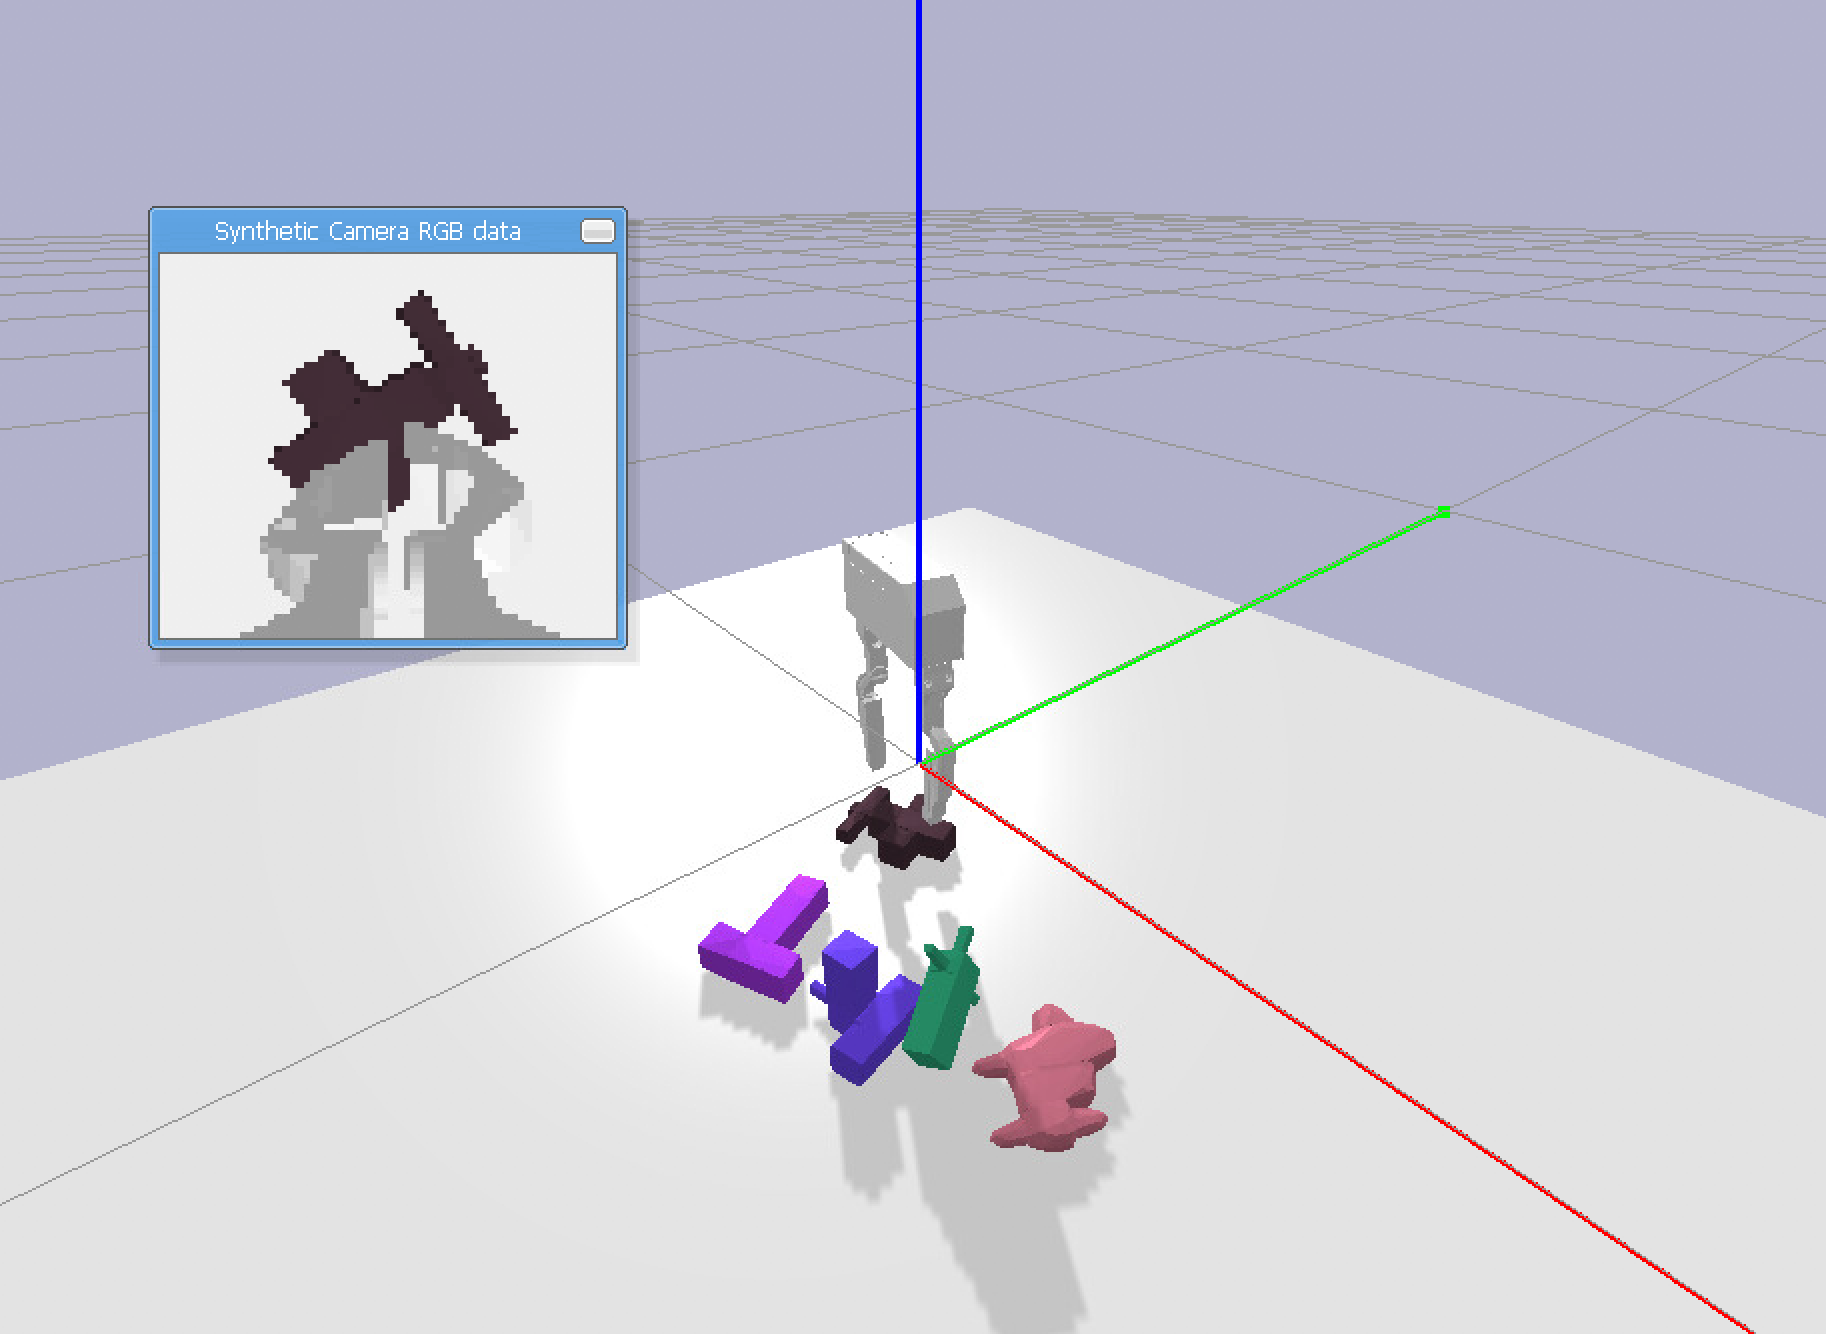
\includegraphics[width=\linewidth]{figures/failure/floorfailure2}
        %         \caption{Floor Scene} \label{fig:floor}
        %     \end{subfigure}%
        %     \hspace*{\fill}   % maximize separation between the subfigures    
        %     \caption{ Table and floor scenes \label{fig:scenes}}
        % \end{figure}
        \begin{figure}[!htbp]
            \begin{subfigure}{0.49\textwidth}
                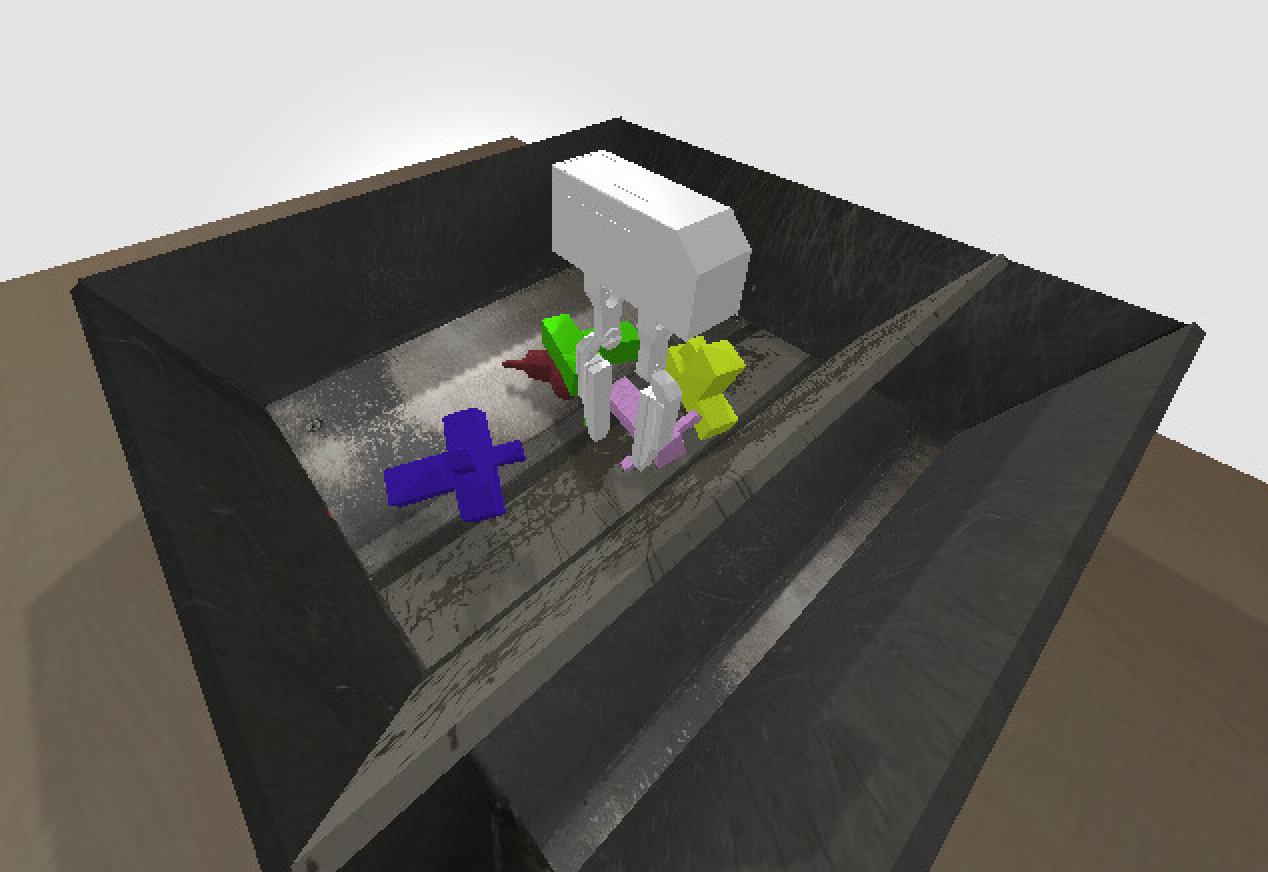
\includegraphics[width=\linewidth]{figures/failure/tablefailure2}
                \caption{Gripper positions itself above the pink object} \label{fig:table}
            \end{subfigure}%
            \hspace*{\fill}   % maximize separation between the subfigures
            \begin{subfigure}{0.49\textwidth}
                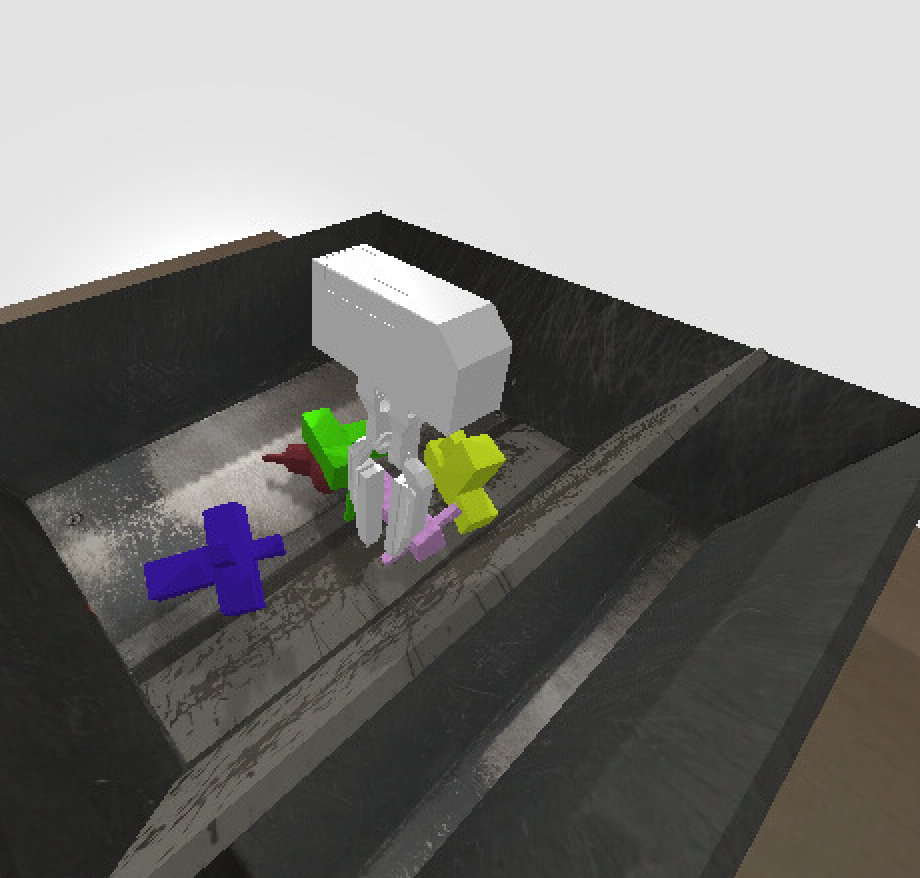
\includegraphics[width=\linewidth]{figures/failure/tablefailure1}
                \caption{Gripper attempts to grasp the pink object unsuccessfully} \label{fig:floor}
            \end{subfigure}%
            \hspace*{\fill}   % maximize separation between the subfigures    
            \caption{ Depth misinterpretation of pink object in the full environment\label{fig:scenes}}
        \end{figure}

    \item \textbf{Grasping the tray's edge} - RGBD or Depth observation types perceive the tray's edge as a graspable object. This misjudgment accounts for up to 50\% of the failed grasp attempts in the table scene \ref{table:SACfull} \ref{fig:failTrayEdge}. We realized that the failure percentage increases when we start the gripper from a higher start point.

    Both observation types tackled the height problem that appeared in the encoder problem. The online nature of these observation types corrected itself when a depth discrepancy occurs. However, it seems that these online observation methods encode the graspable objects' features very similar to other household objects. This characteristic can be interpreted both positively and negatively. It is positive because the perception layer extrapolates the graspable features correctly from the trained objects and applies it to the tray object. It can be viewed negatively because the tray is not our target object; eventually, the gripper should differentiate between the targeted objects and the extra tray object.   
    
    This failure mode can be solved by training the trained model for a short time in the table scene. This procedure should suffice for the agent to understand that tray is not the targeted object.
    \begin{figure}[!htbp]
        \begin{subfigure}{0.33\textwidth}
            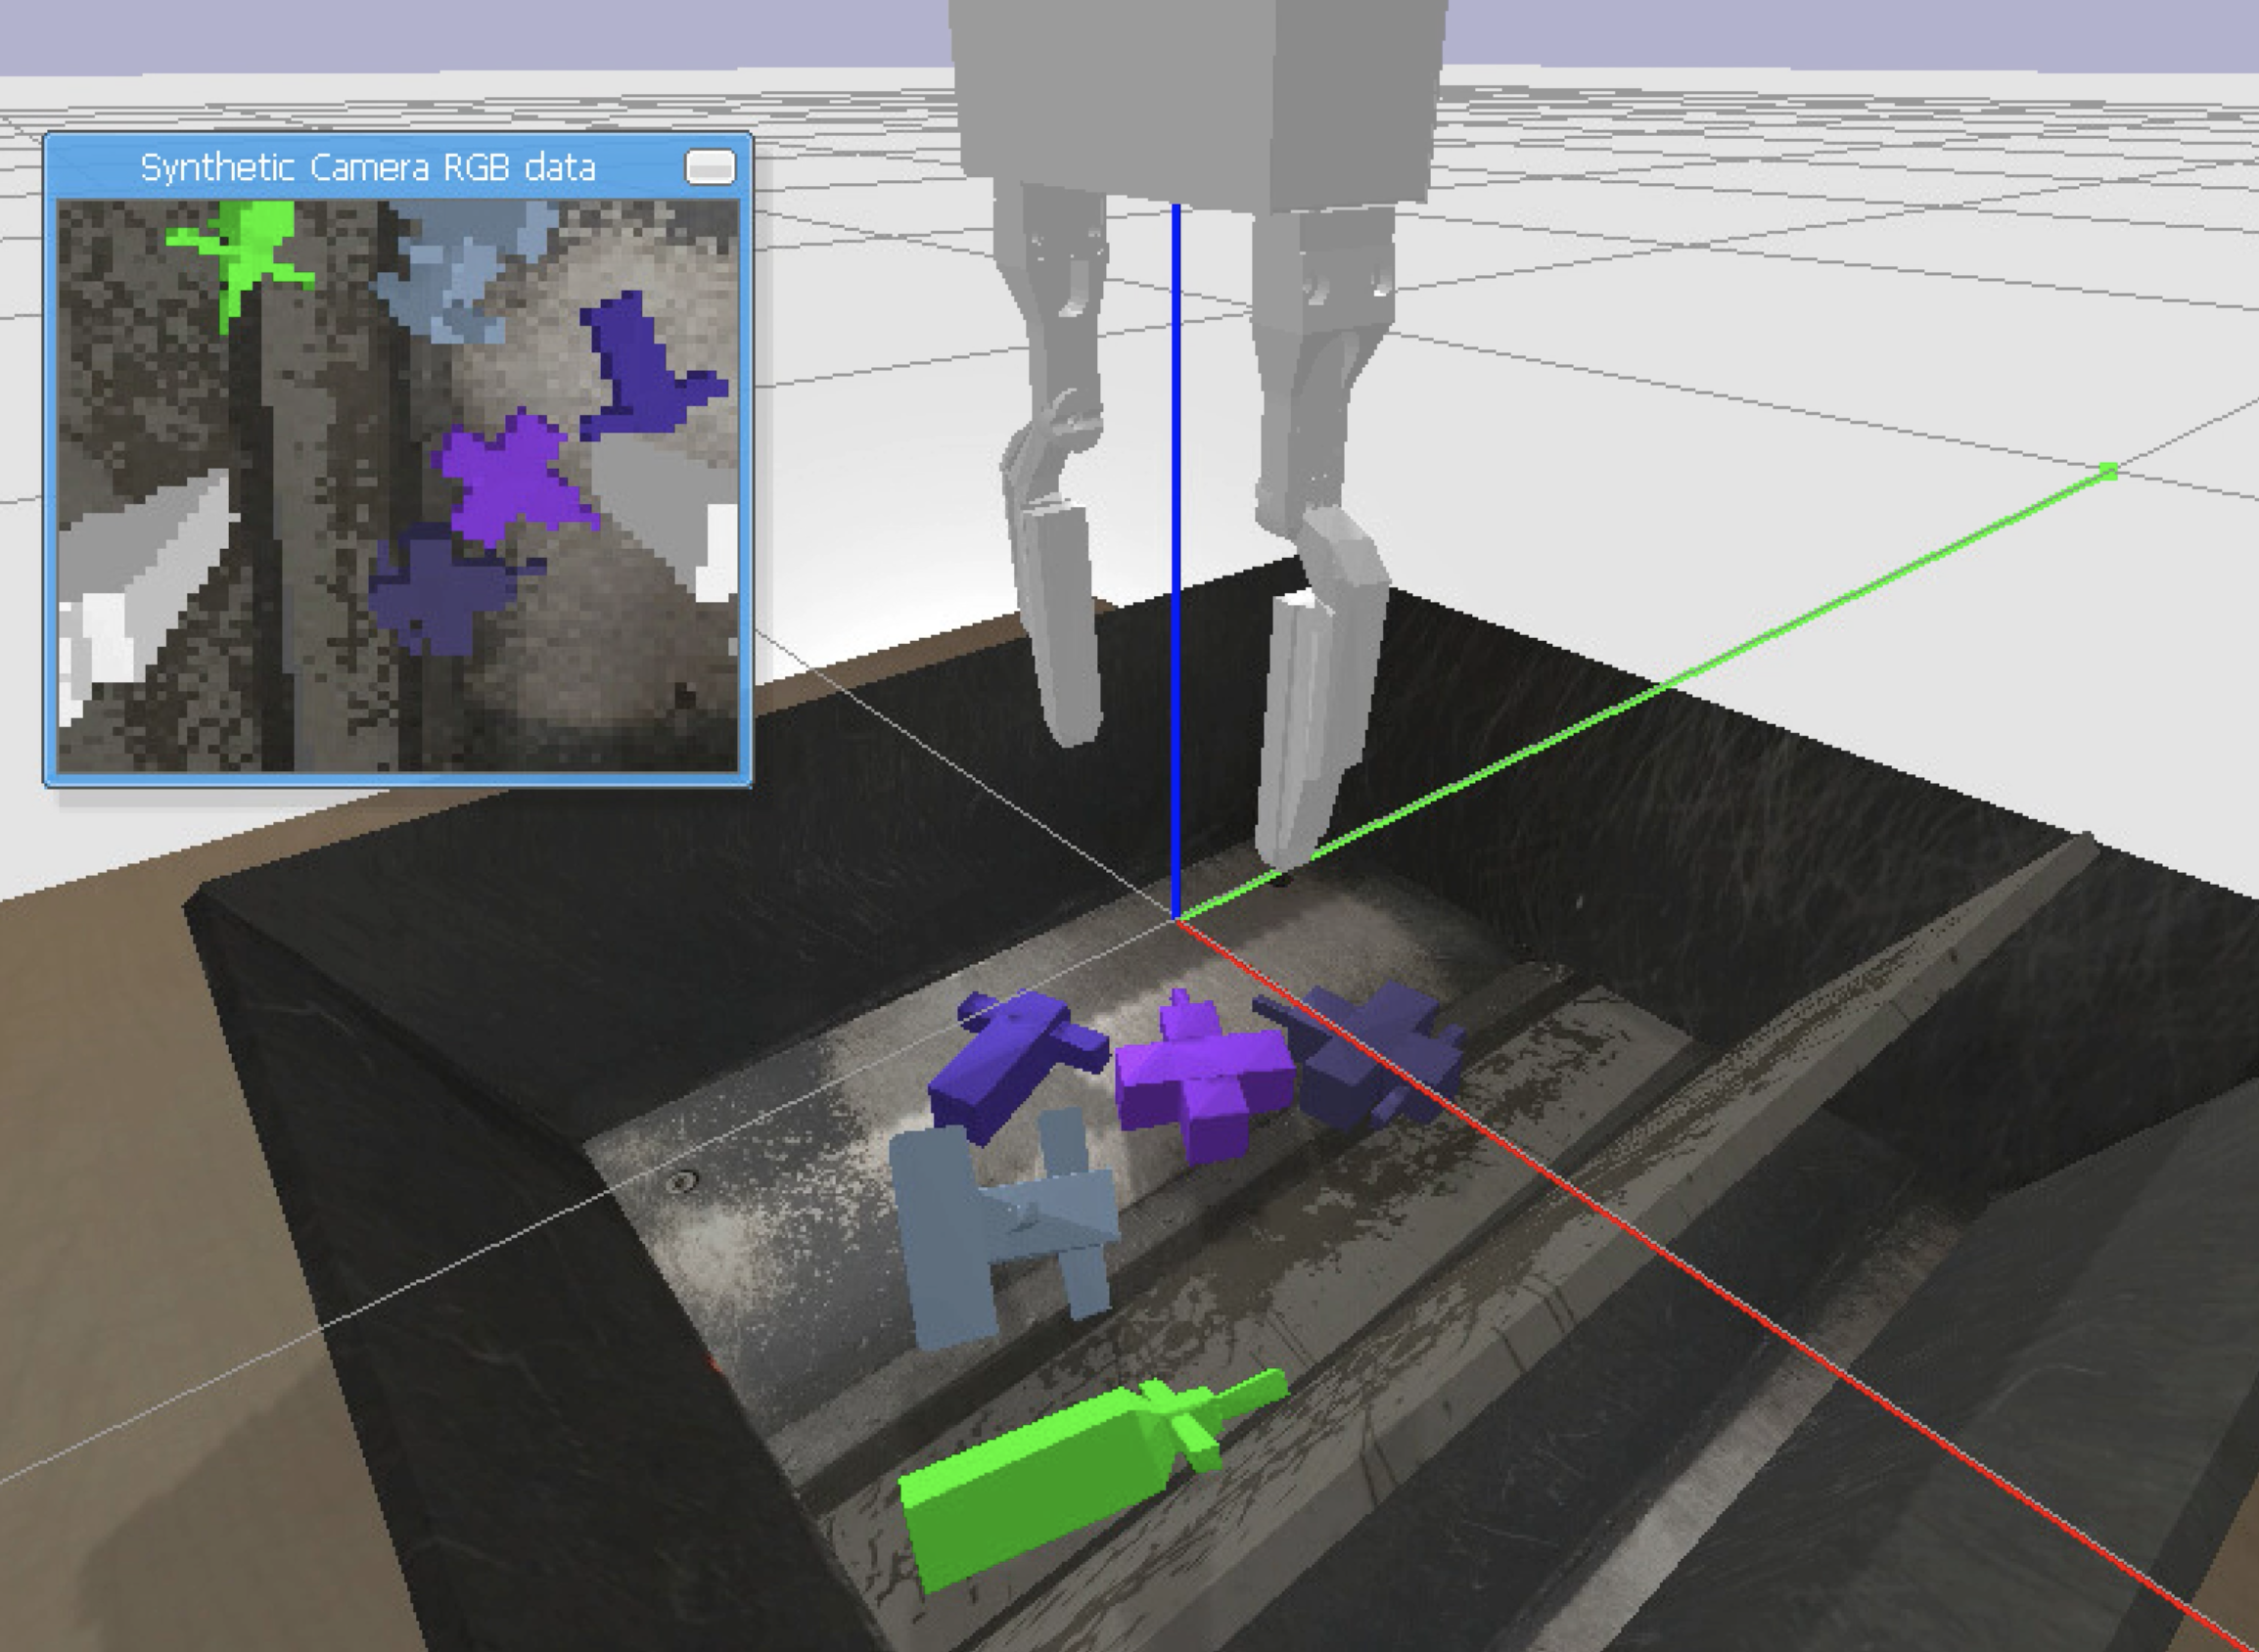
\includegraphics[width=\linewidth]{figures/failure/trayedge1}
            \caption{Gripper starts the movement to the tray's edge} \label{fig:table}
        \end{subfigure}%
        \hspace*{\fill}   % maximize separation between the subfigures
        \begin{subfigure}{0.35\textwidth}
            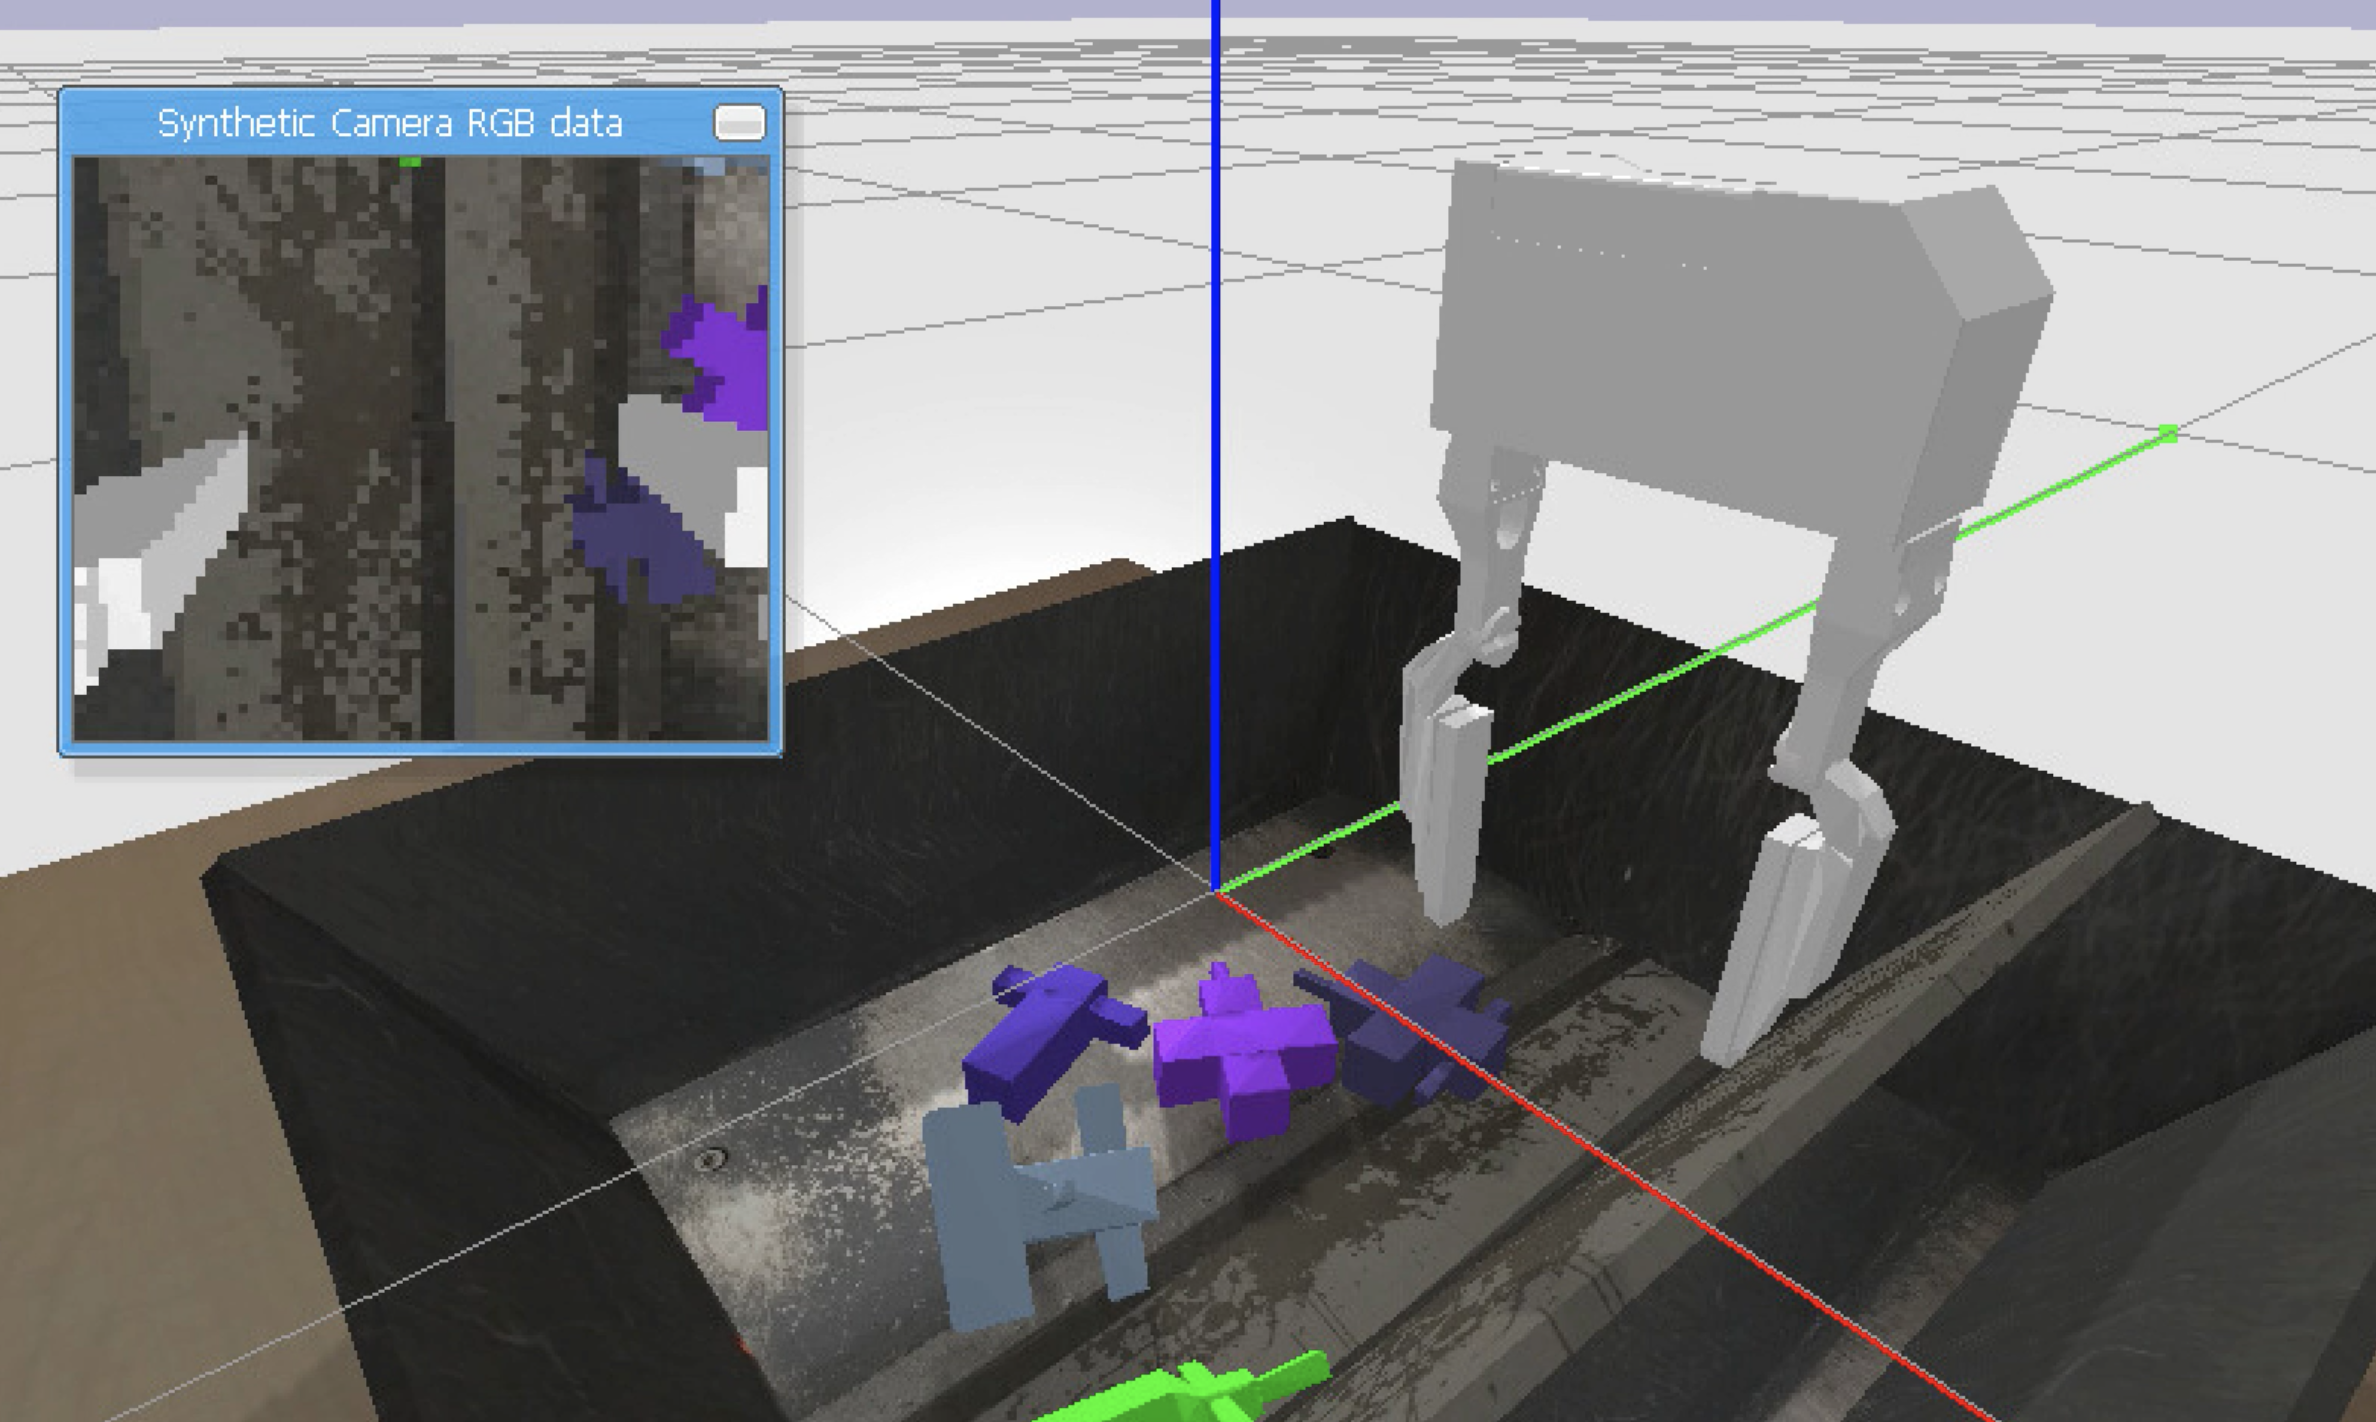
\includegraphics[width=\linewidth]{figures/failure/trayedge2}
            \caption{Gripper positions itself just above the tray's edge} \label{fig:floor}
        \end{subfigure}%
        \hspace*{\fill}   % maximize separation between the subfigures    
        \begin{subfigure}{0.33\textwidth}
            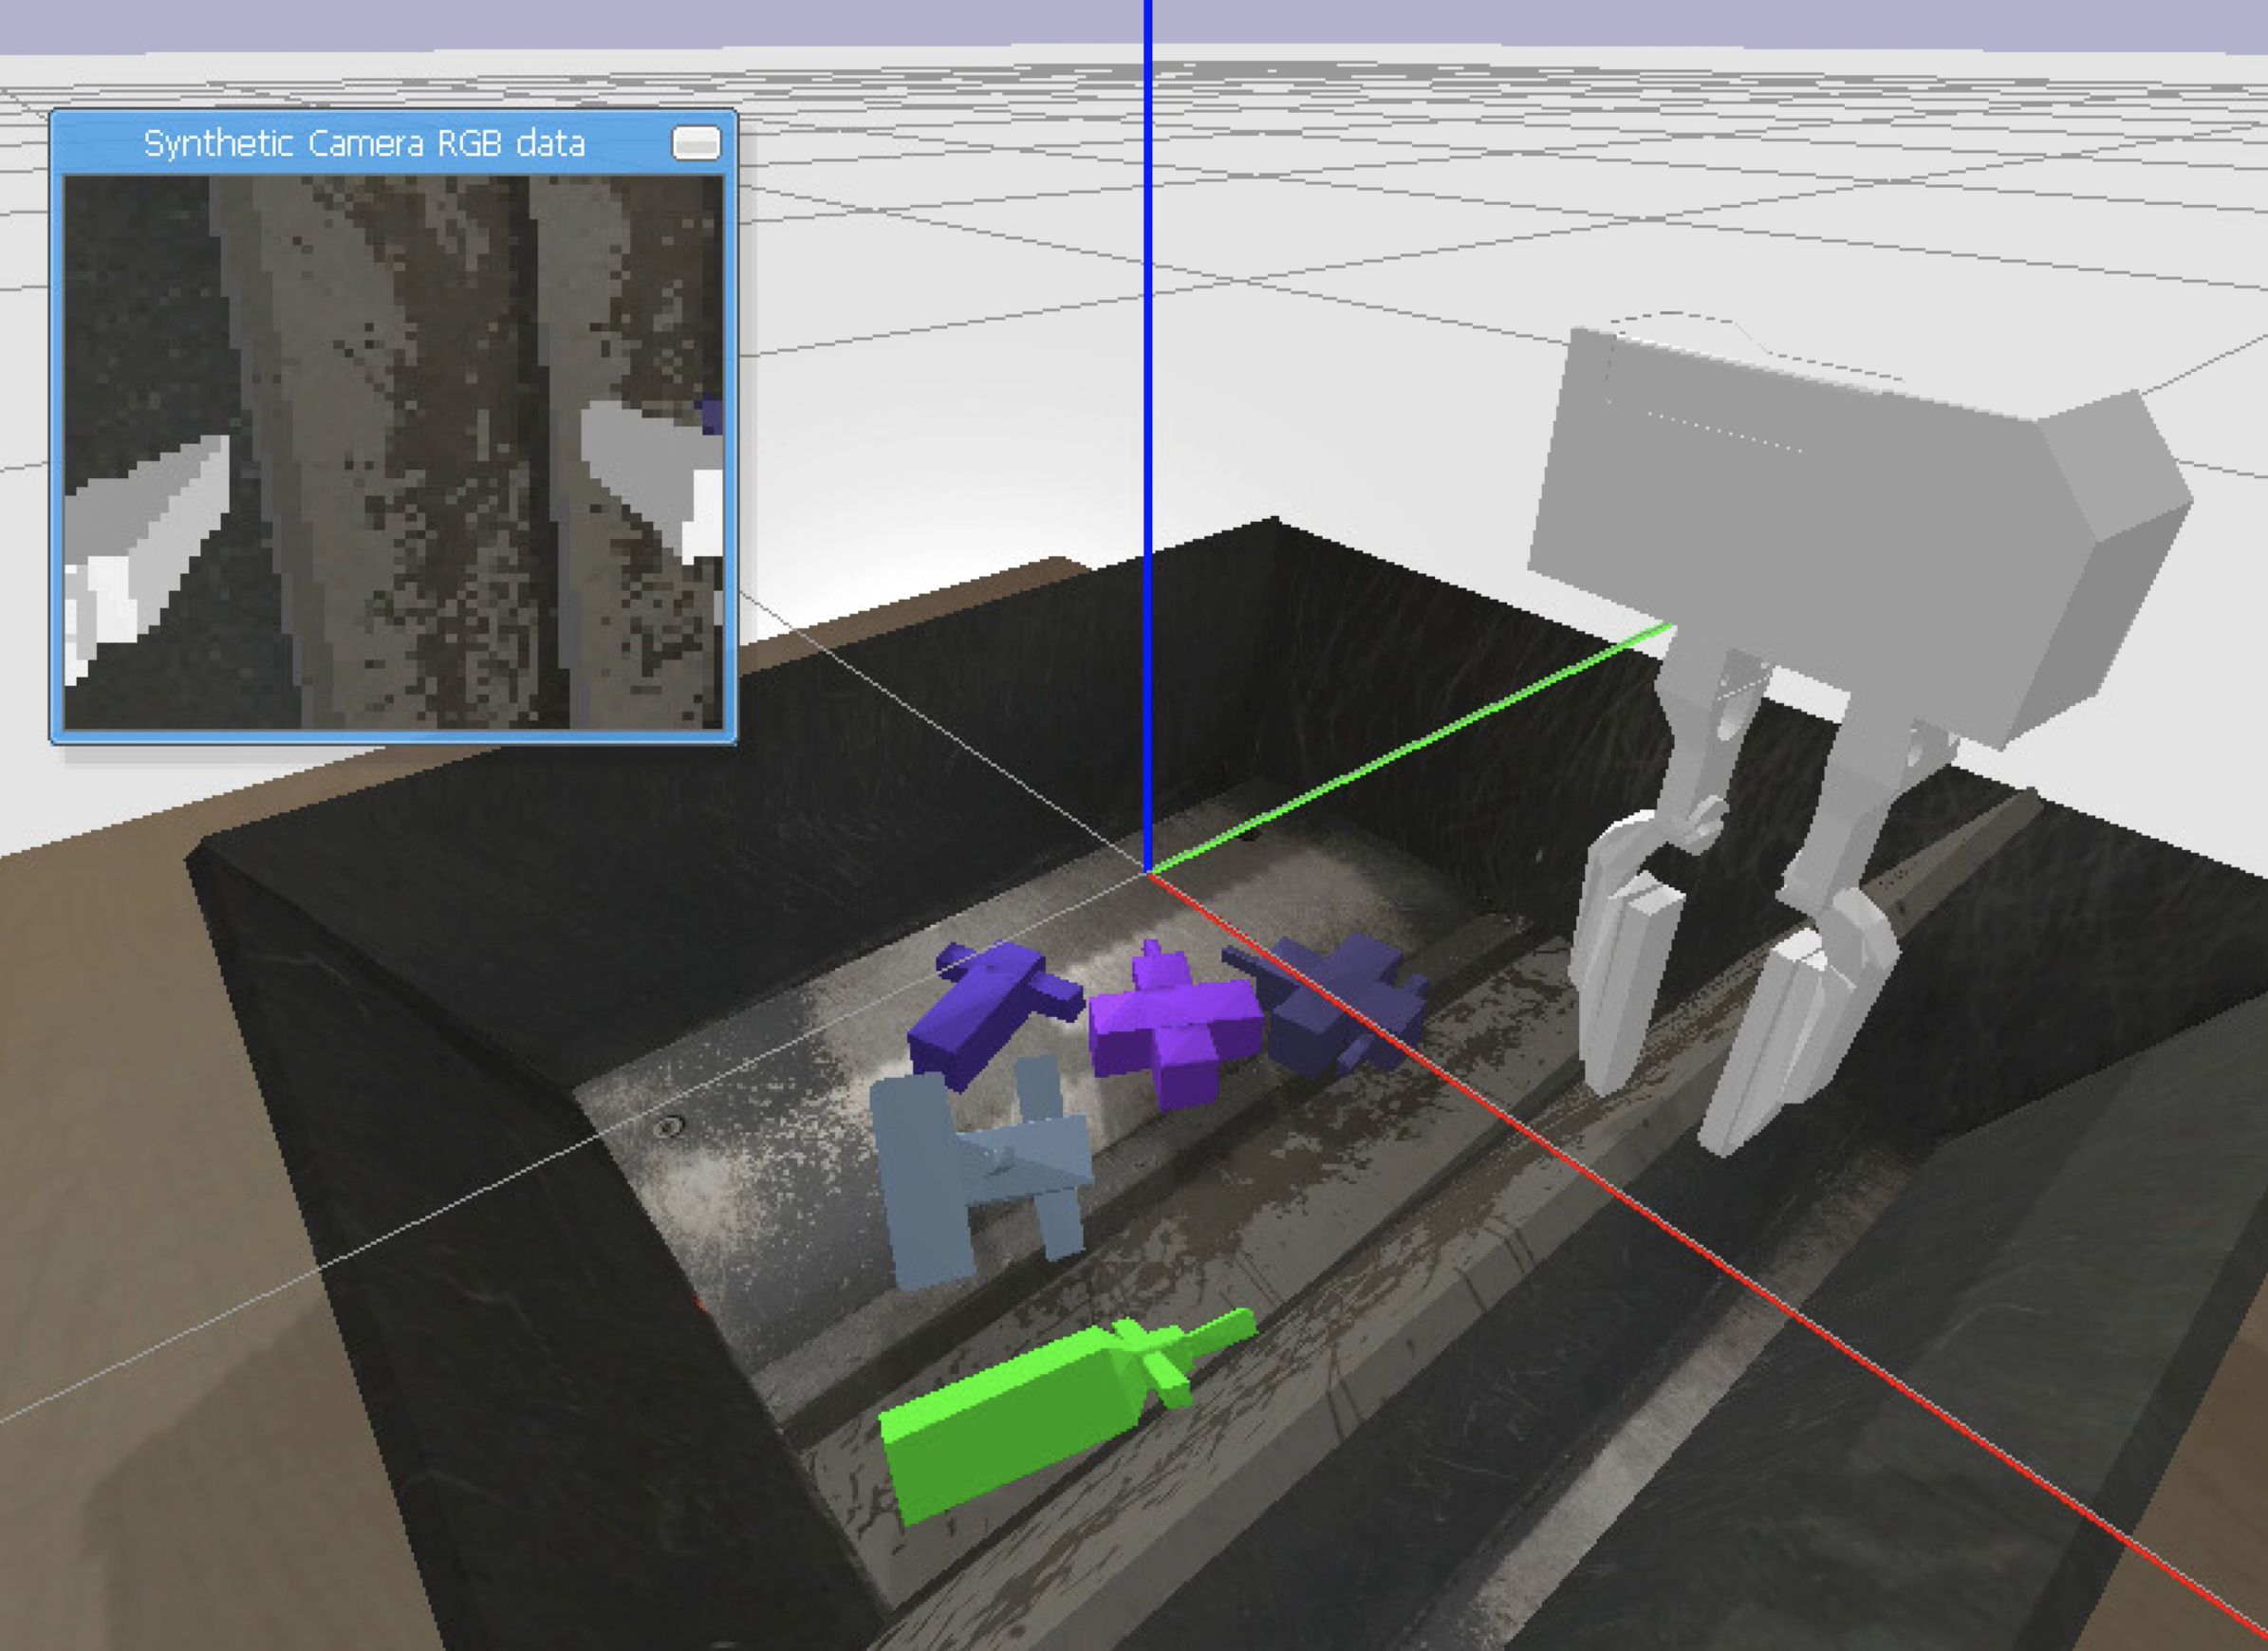
\includegraphics[width=\linewidth]{figures/failure/trayedge3}
            \caption{Gripper grasps the tray's edge} \label{fig:floor}
        \end{subfigure}%
        \hspace*{\fill}   % maximize separation between the subfigures    
        \caption{Sequence of movement to the tray's edge\label{fig:failTrayEdge}}
    \end{figure} 

\end{enumerate}